\documentclass[final]{beamer}
\mode<presentation> {  %% check http://www-i6.informatik.rwth-aachen.de/~dreuw/latexbeamerposter.php for examples
  \usetheme{I6pd}    %% you should define your own theme e.g. for big headlines using your own logos 
}
\usepackage[english]{babel}
\usepackage[latin1]{inputenc}
\usepackage{amsmath,amsthm, amssymb, latexsym}
\usepackage{graphicx}
\usepackage{array,booktabs,tabularx}
\usefonttheme[onlymath]{serif}
\boldmath
\usepackage[orientation=landscape,size=custom,width=200,height=120,scale=2,debug]{beamerposter}
\title{\huge Reproducible Proteomic Workflows using Extensions to the Galaxy Framework}
\author[Johnson, Chilton, et al]{James Johnson; John Chilton; Pratik Jagtap; Ben Lynch; Tim Griffin}
\institute[]{University of Minnesota Supcomputing Institute}
\date{June 10th, 2013}

\newlength{\columnheight}
\setlength{\columnheight}{105cm}

\begin{document}
\begin{frame}
  \begin{columns}

    \begin{column}{.33\textwidth}
      \begin{beamercolorbox}[center,wd=\textwidth]{postercolumn}
        \begin{minipage}[T]{.95\textwidth}  % tweaks the width, makes a new \textwidth
          \parbox[t][\columnheight]{\textwidth}{
            \begin{block}{Introduction}


            \end{block}
            \vfill
          }
        \end{minipage}
      \end{beamercolorbox}
    \end{column}

    \begin{column}{.33\textwidth}
      \begin{beamercolorbox}[center,wd=\textwidth]{postercolumn}
        \begin{minipage}[T]{.95\textwidth} % tweaks the width, makes a new \textwidth
          \parbox[t][\columnheight]{\textwidth}{
            \begin{block}{Challenge - Handling Large Numbers of Files}

            From Wikipedia, "[Galaxy design choices make] it relatively easy
            to build typical analyses, but more difficult to build complex
            workflows..."

            The common use of fractionation, means the problem is that typical
            analyses in Proteomics are relatively complex structurally
            relative to Genomics. Galaxy is not geared toward handling large
            numbers of files.

            \end{block}
            \vfill
            \begin{block}{Handling Large Numbers of Files - JGalaxy}

            
            \begin{columns}
              \begin{column}{.55\textwidth}
              We developed a Java Web Start rich client application called
              JGalaxy targetting the Galaxy API to allow easy batch file
              downloads.  
              \end{column}              
              \begin{column}{.44\textwidth}
                \begin{figure}
                  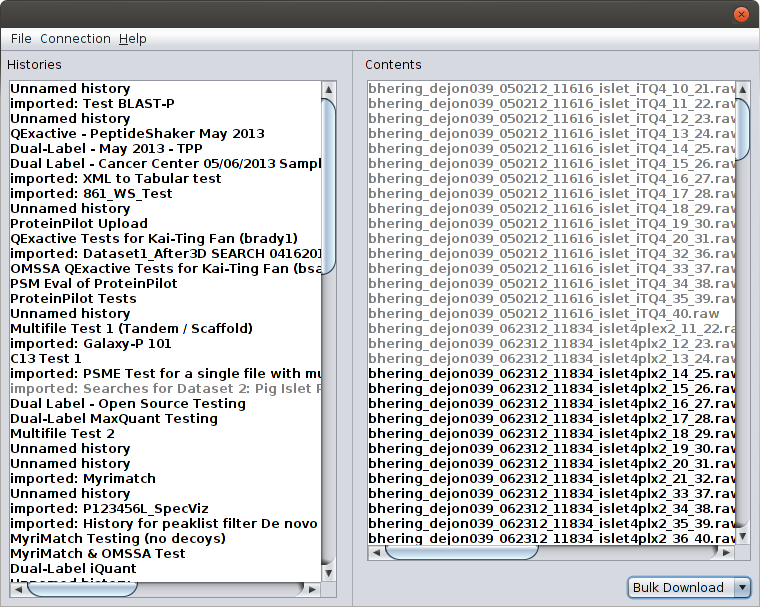
\includegraphics[scale=0.5]{bulkdownload_jgalaxy.png}
                \end{figure}              
              \end{column}
            \end{columns}
            
            \end{block}
            \vfill
            \begin{block}{Handling Large Numbers of Files - Tool Extensions}

            \end{block}
            \vfill
            \begin{block}{Handling Large Numbers of Files - Multiple File Datasets}

            \end{block}
            \vfill
            \begin{block}{Handling Large Numbers of Files - Multiple File Datasets}

            \end{block}
            \vfill
          }
        \end{minipage}
      \end{beamercolorbox}
    \end{column}              

    \begin{column}{.33\textwidth}
      \begin{beamercolorbox}[center,wd=\textwidth]{postercolumn}
        \begin{minipage}[T]{.95\textwidth} % tweaks the width, makes a new \textwidth
          \parbox[t][\columnheight]{\textwidth}{
            \begin{block}{Cross Platform Job Execution - Challenges}

            Perhaps driven by proprietary data formats, proteomics has a
            Windows-centric culture not present in genomics. As an upshot,
            previously there was no easy way to run Windows applications in
            the Galaxy framework.

            % Make Bigger!
            The large number of important proteomics applications tied to the
            Windows platform nesseciatated the creation of the LWR.


            \end{block}
            \vfill
            \begin{block}{Cross Platform Job Execution with the LWR}

            The LWR is an application that can be installed on any server
            (Windows or *nix) and allows a remote Galaxy instance to submit
            jobs to that host.

            \begin{itemize}
            \item https://lwr.readthedocs.org - Read more about installing the LWR and configuring Galaxy clients 
            \item https://bit.ly/galaxy-lwr-code - Check out the LWR source code.
            \end{itemize}

            \end{block}
            \vfill
            \begin{block}{Cross Platform Tool - msconvert}
              \begin{figure}
                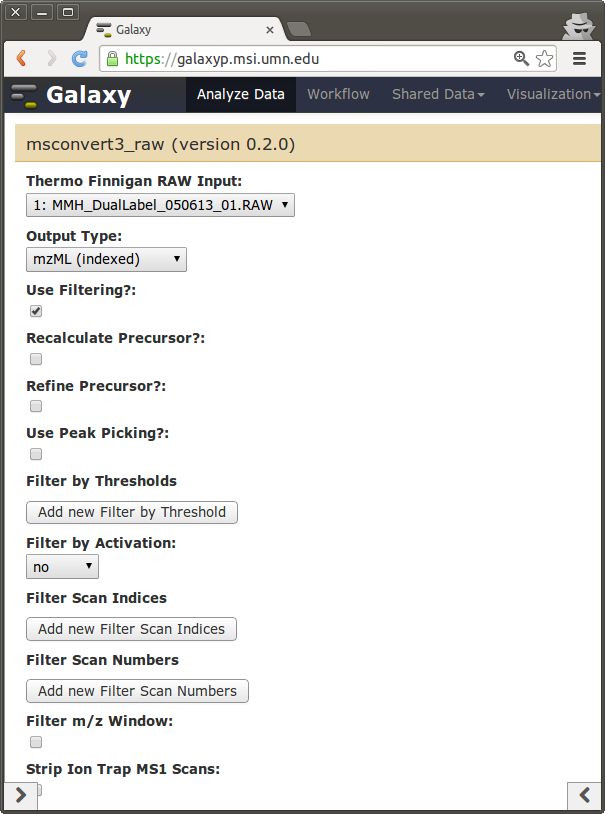
\includegraphics[scale=0.5]{msconvert3_screenshot.png}
              \end{figure}
            \end{block}
            \vfill
            \begin{block}{Cross Platform Tool - maxquant}
              \begin{figure}
                \includegraphics[scale=0.5]{maxquant_screenshot.png}
              \end{figure}
            \end{block}
            \vfill
            \begin{block}{Cross Platform Tool - proteinpilot}
              \begin{figure}
                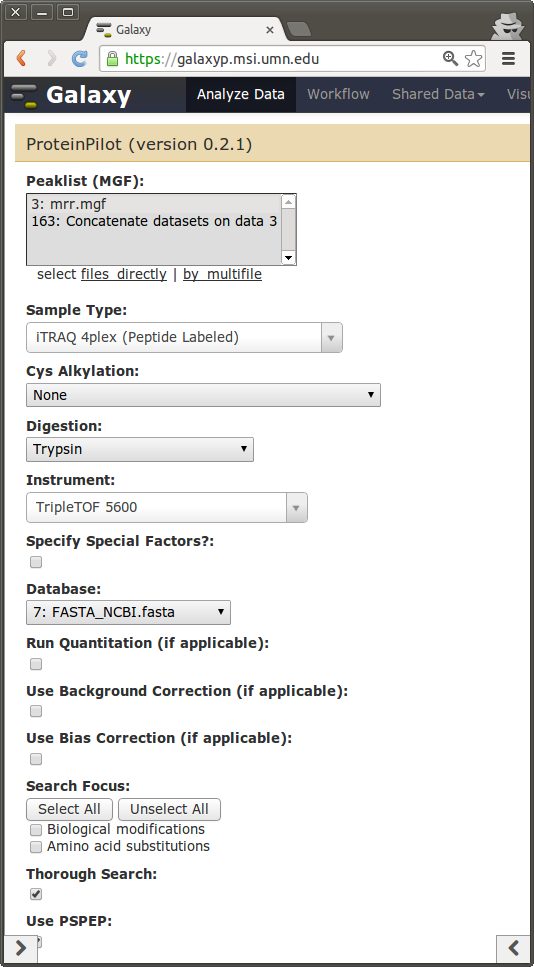
\includegraphics[scale=0.5]{proteinpilot_screenshot.png}
              \end{figure}
            \end{block}
            \vfill
          }
        \end{minipage}
      \end{beamercolorbox}
    \end{column}              



  \end{columns}   
\end{frame}
\end{document}
